\documentclass[tikz,border=10pt]{standalone}
% Scale follows STYLE METRICS (s = 0.021333 cm/px), so the figure spans 8 cm.
\begin{document}
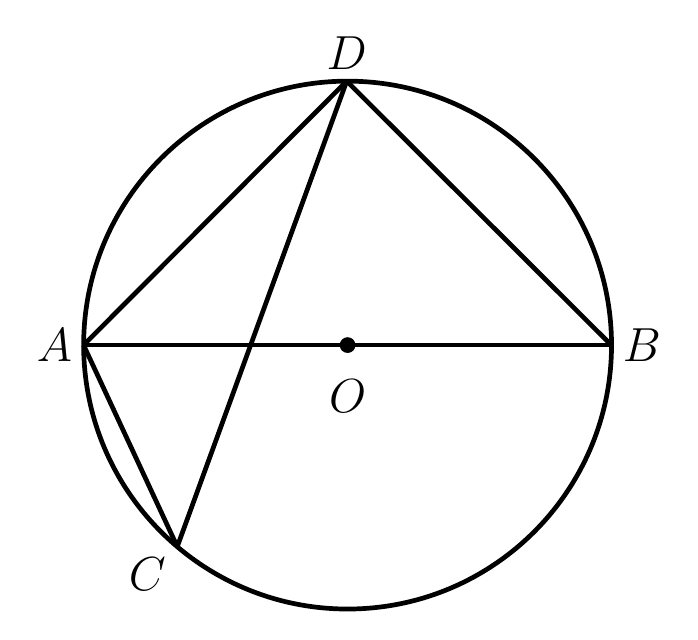
\begin{tikzpicture}[line join=round, line width=1.7pt, font=\fontsize{18}{21.6}\selectfont]
  % Named coordinates: O centre, pixels relative to O, y flipped
  \coordinate (O) at (0,0);
  \coordinate (A) at (-3.353,0);
  \coordinate (B) at (3.349,0);
  \coordinate (D) at (-0.011,3.352);
  \coordinate (C) at (-2.163,-2.560);

  % Circle of radius 157.1 px (3.352 cm)
  \draw (O) circle[radius=3.352];

  % Diameter and chords
  \draw (A) -- (B);
  \draw (A) -- (D);
  \draw (D) -- (B);
  \draw (A) -- (C);
  \draw (C) -- (D);

  % Centre dot: filled circle, radius about 0.1 cm
  \fill (O) circle[radius=0.1];

  % Labels
  \node[left]        at (A) {$A$};
  \node[right]       at (B) {$B$};
  \node[above]       at (D) {$D$};
  \node[below left]  at (C) {$C$};
  % O label: anchor north, placed about 0.3 cm below the dot centre
  % (plain coordinate used instead of calc shorthand, so no library is needed)
  \node[anchor=north] at (0,-0.3) {$O$};
\end{tikzpicture}
\end{document}